\documentclass[11pt,]{article}
\usepackage[T1]{fontenc}
\usepackage{amssymb,amsmath}
\usepackage{txfonts}
\usepackage{microtype}
\usepackage{amssymb,amsmath}
\usepackage{graphicx}
\usepackage{subfigure} 
\usepackage{natbib}
\usepackage{paralist}
\usepackage{hyperref}
\usepackage{url}
\urlstyle{same}
\usepackage{color}
\usepackage{fancyvrb}
\usepackage[a4paper,body={170mm,250mm},top=25mm,left=25mm,head=14pt]{geometry}
\usepackage[sf,bf,small]{titlesec}
\usepackage{fancyhdr}
\usepackage{todonotes}

\renewcommand*\ttdefault{txtt} % 20% tighter than courier

%% uses fancyvrb
\newcommand{\VerbBar}{|}
\newcommand{\VERB}{\Verb[commandchars=\\\{\}]}
\DefineVerbatimEnvironment{Highlighting}{Verbatim}{commandchars=\\\{\}}
% Add ',fontsize=\small' for more characters per line

\newenvironment{Shaded}{}{}
\newcommand{\KeywordTok}[1]{\textcolor[rgb]{0.00,0.44,0.13}{\textbf{{#1}}}}
\newcommand{\DataTypeTok}[1]{\textcolor[rgb]{0.56,0.13,0.00}{{#1}}}
\newcommand{\DecValTok}[1]{\textcolor[rgb]{0.25,0.63,0.44}{{#1}}}
\newcommand{\BaseNTok}[1]{\textcolor[rgb]{0.25,0.63,0.44}{{#1}}}
\newcommand{\FloatTok}[1]{\textcolor[rgb]{0.25,0.63,0.44}{{#1}}}
\newcommand{\CharTok}[1]{\textcolor[rgb]{0.25,0.44,0.63}{{#1}}}
\newcommand{\StringTok}[1]{\textcolor[rgb]{0.25,0.44,0.63}{{#1}}}
\newcommand{\CommentTok}[1]{\textcolor[rgb]{0.38,0.63,0.69}{\textit{{#1}}}}
\newcommand{\OtherTok}[1]{\textcolor[rgb]{0.00,0.44,0.13}{{#1}}}
\newcommand{\AlertTok}[1]{\textcolor[rgb]{1.00,0.00,0.00}{\textbf{{#1}}}}
\newcommand{\FunctionTok}[1]{\textcolor[rgb]{0.02,0.16,0.49}{{#1}}}
\newcommand{\RegionMarkerTok}[1]{{#1}}
\newcommand{\ErrorTok}[1]{\textcolor[rgb]{1.00,0.00,0.00}{\textbf{{#1}}}}
\newcommand{\NormalTok}[1]{{#1}}

\hypersetup{breaklinks=true,
            pdfauthor={},
            pdftitle={},
            colorlinks=true,
            citecolor=blue,
            urlcolor=blue,
            linkcolor=magenta,
            pdfborder={0 0 0}}

\setlength{\parindent}{0pt}
\setlength{\parskip}{6pt plus 2pt minus 1pt}
\setlength{\emergencystretch}{3em}  % prevent overfull lines

\newcommand{\todo}[2]{{\textcolor{red}{\bf [#1] #2 }}\addcontentsline{toc}{subsubsection}{\textcolor{red}{[#1] #2} }}
\newcommand{\notes}[1]{\textcolor{blue}{\it #1 }}

\DeclareMathOperator{\softmax}{softmax}
\DeclareMathOperator{\sigmoid}{sigmoid}
\DeclareMathOperator{\sgn}{sgn}
\DeclareMathOperator{\relu}{relu}
\DeclareMathOperator{\lrelu}{lrelu}
\DeclareMathOperator{\elu}{elu}
\DeclareMathOperator{\selu}{selu}
\DeclareMathOperator{\maxout}{maxout}


%% uses fancyhdr
\pagestyle{fancy}

\author{}
\date{}



%% uses fancyhdr
\lhead{\sffamily MLP 2020/21:  Coursework 1}
\rhead{\sffamily Due: 30 October 2020}
\cfoot{\sffamily \thepage}
% \usepackage{subcaption}
% \usepackage{caption}
\begin{document}

\begin{center}
\textsf{\textbf{\Large Machine Learning Practical 2020/21: Coursework 1}}

\bigskip
\textbf{Released: Monday 19 October 2020}

\textbf{Submission due: 16:00 Friday 30 October 2020}
\end{center}
\section{Introduction}
\label{sec:introduction}

The aim of this coursework is to explore the classification of images of handwritten digits using neural networks. 
The first part of this coursework will concern the identification and discussion of a \textit{fundamental problem} in machine learning, as shown in Figure~\ref{fig:errorfn}. 
Following this preliminary discussion, you will further investigate this problem in \textit{wider} and \textit{deeper} neural networks, study it in terms of network width and depth. 
The second part involves implementing different methods to combat the problem identified in Task 1 and then comparing these methods empirically and theoretically. 
In the final part, you will briefly discuss the main strengths and weakness of any one related work to the methods examined in Task 2. 

The coursework will use an extended version of the MNIST database, the EMNIST Balanced dataset, described in Section~\ref{sec:emnist}.  Section \ref{sec:code} describes the additional code provided for the coursework (in branch \texttt{mlp2020-21/coursework\_1} of the MLP github), and Section \ref{sec:tasks} describes how the coursework is structured into three tasks. 
The main deliverable of this coursework is a report, discussed in section \ref{sec:report}, using a template that is available on the github. 
Section \ref{sec:mechanics} discusses the details of carrying out and submitting the coursework, and the marking scheme is discussed in Section \ref{sec:marking-scheme}.

You will need to submit your completed report as a PDF file  and your local version of the \texttt{mlp} code including any changes you made to the provided (\texttt{.py} files).  
The detailed submission instructions are given in Section \ref{sec:submission} -- please follow these instructions carefully.

\section{EMNIST dataset}
\label{sec:emnist}
In this coursework we shall use the  EMNIST  (Extended MNIST) Balanced dataset \citep{cohen2017emnist}, \url{https://www.nist.gov/itl/iad/image-group/emnist-dataset}. EMNIST extends MNIST by including images of handwritten letters (upper and lower case) as well as handwritten digits. Both EMNIST and MNIST are extracted from the same underlying dataset, referred to as NIST Special Database 19.  Both use the same conversion process resulting in centred images of dimension 28$\times$28.  

There are 62 potential classes for EMNIST (10 digits, 26 lower case letters, and 26 upper case letters).  However, we shall use a reduced label set of 47 different labels.  This is because (following the data conversion process)  there are 15 letters for which it is confusing to discriminate between upper-case and lower-case versions.  In the 47 label set, upper- and lower-case labels are merged for the following letters:\\
\texttt{C, I, J, K, L, M, O, P, S, U, V, W, X, Y, Z}.  

The training set for Balanced EMNIST has about twice the number of examples as the MNIST training set, thus you should expect the run-time of your experiments to be about twice as long.  The expected accuracy rates are lower for EMNIST than for MNIST (as EMNIST has more classes, and more confusable examples), and differences in accuracy between different systems should be larger. \citet{cohen2017emnist} present some baseline results for EMNIST.

You do \emph{not} need to directly download the EMNIST database from the \href{https://www.nist.gov/itl/iad/image-group/emnist-dataset}{nist.gov} website, as it is part of the \verb+coursework_1+ branch in the \verb+mlpractical+ Github repository,  discussed in Section~\ref{sec:code} below.

\newpage
\section{Github branch \texttt{mlp2020-21/coursework\_1}}
\label{sec:code}

You should run all of the experiments for the coursework inside the Conda environment you set up for the labs. The code for the coursework is available on the course \href{https://github.com/VICO-UoE/mlpractical/}{Github repository} on a branch \verb+mlp2020-21/coursework_1+. 
To create a local working copy of this branch in your local repository you need to do the following.

\begin{enumerate}
\def\labelenumi{\arabic{enumi}.}
\itemsep3pt\parskip0pt\parsep0pt
\item Make sure all modified files on the branch you are currently have been committed
  (see \href{https://github.com/VICO-UoE/mlpractical/blob/mlp2020-21/lab1/notes/getting-started-in-a-lab.md}{notes/getting-started-in-a-lab.md} if you are unsure how to do this).
\item Fetch changes to the upstream \texttt{origin} repository by running\\
  \texttt{git fetch origin}
\item Checkout a new local branch from the fetched branch using\\
  \verb+git checkout -b coursework_1 origin/mlp2020-21/coursework_1+
\end{enumerate}

You will now have a new branch in your local repository with all the code necessary for the coursework in it.   

This branch includes the following additions to your setup:

\begin{itemize}
	\item A new \texttt{EMNISTDataProvider} class in the \verb+mlp.data_providers+ module.
	This class makes some changes to the \texttt{MNISTDataProvider} class, linking to the \texttt{EMNIST Balanced} data, and setting the number of classes to 47.
	\item Training, validation, and test sets for the \texttt{EMNIST Balanced} dataset that
	you will use in this coursework.
	\item In order to further improve performance and mitigate the problem identified in neural networks, you will also need to implement a new class in the \verb+mlp.layers+ module:\\
 	\texttt{DropoutLayer}\\
 	and also two weight penalty tecniques in the \verb+mlp.penalties+ module:\\
	\texttt{L1Penalty and L2Penalty}. 
	\item \texttt{DropoutandPenalty\_tests.ipynb} Jupyter notebook\\
	to be used for testing the implementations of {\texttt{{DropoutLayer}}}, {\texttt{L1Penalty and L2Penalty}} classes. The tests serve as a safeguard to prevent experimentation with faulty code which might lead to wrong conclusions. Tests in general are a \emph{vital} ingredient for good software development, and especially important for building correct and  efficient deep learning systems. 
	
	\textbf{Please note} that passing these preliminary tests \textit{does not} necessarily mean your classes are absolutely bug-free. If you get unexpected curves during model training, re-check your implementation of the classes. 
	
	\item A directory called \texttt{report} which contains the LaTeX template and style files for your report.  You should copy all these files into the directory which will contain your report.
\end{itemize}



\newpage
\section{Tasks}
\label{sec:tasks}
The coursework is structured into 3 tasks, the first two are supported by experiments on \texttt{EMNIST} dataset. 
\begin{enumerate}
    \item Identification of a fundamental problem in machine learning as shown in Fig \ref{fig:errorfn} and setting up a \textbf{baseline} system on \texttt{EMNIST} by a valid hyper-parameter search. 
   
    \item A research investigation and analysis into whether using Dropout and/or Weight Penalty (\texttt{L1Penalty} and \texttt{L2Penalty}) addresses the problem found in training machine learning models (Fig \ref{fig:errorfn}). How do these two approaches improve/degrade the model's performance?
    \item{A brief literature review of any one work as discussed in Section \ref{sec:part3}.}
\end{enumerate}



\section{Task 1: Problem identification}
\label{sec:baseline}


\begin{figure}
% \begin{center}
\centering

\begin{subfigure}{.8\textwidth}
\centering

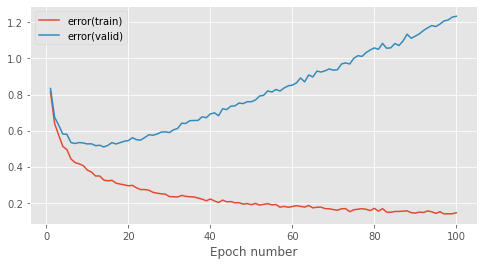
\includegraphics[width=0.75\linewidth]{error_IHO_withrelu.png}
\caption{Error curve on the training and validation set of EMNIST dataset.} 
\label{fig:error}
\end{subfigure}
% \end{center}
% \begin{center}
\centering

\begin{subfigure}{.8\textwidth}
\centering

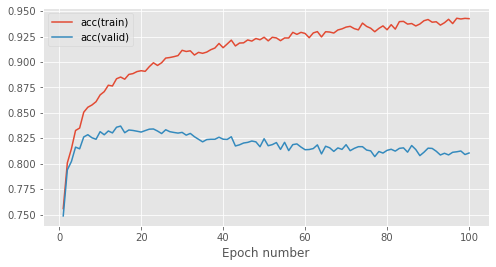
\includegraphics[width=0.8\linewidth]{accuracy_IHO_withrelu.png}
\caption{Accuracy curve on the training and validation set of EMNIST dataset.}

\label{fig:accuracy}
\end{subfigure}
\caption{Error and Accuracy curves for a baseline model on EMNIST Dataset.}
\label{fig:errorfn}

\end{figure}

Figure~\ref{fig:errorfn} shows the training and validation error curves in Figure~\ref{fig:error} and also training and validation accuracies in Figure~\ref{fig:accuracy} for a model with 1 hidden layer and a ReLU activation function trained on the EMNIST dataset by using cross-entropy error function. 
This curve can be re-produced by running the model settings defined in the \texttt{Coursework1.ipynb} notebook in the github repository.
First identify and discuss the problem shown by the curves in Figure~\ref{fig:errorfn} and briefly discuss potential solutions in this section for overcoming this problem.

\textbf{Varying number of hidden units.} Initially you will train various 1-hidden layer networks by using either 32, 64 and 128 ReLU hidden units per layer on \texttt{EMNIST} using stochastic gradient descent (SGD) without any regularization.
Make sure you use an appropriate learning rate and train each network for 100 epochs.
Visualise and discuss how increasing number of hidden units affects the validation performance and whether it worsens or mitigates the problem. 

\emph{(10 Marks)}
% Initially you need to establish a baseline system on \texttt{EMNIST} using stochastic gradient descent (SGD) and without explicit regularization.
% Design different models by varying number of ReLU hidden units per layer and number of layers.
% Carry out experiments using 32, 64 and 128 ReLU hidden units per layer, and investigate using from 1-3 hidden layers. 
%Make sure you use an appropriate learning rate. 
% Train for 100 epochs. For model selection, you are free to use early stopping to choose the best validation model. Compare systems using the test set accuracy on the model selected above. 

\textbf{Varying number of layers.} Here you will train various neural networks by using either 1, 2, 3 hidden layers with 128 ReLU hidden units per layer on \texttt{EMNIST} using stochastic gradient descent (SGD) without any regularization.
Make sure you use an appropriate learning rate and train each network for 100 epochs.
Visualise and discuss how increasing number of layers affects the validation performance and whether it worsens or mitigates the problem.

\emph{(10 Marks)}




\section{Task 2: Mitigating the problem with Dropout and Weight Penalty}
\label{sec:part2}

\textbf{Definition and Motivation. } Here you will explain 
\begin{itemize}
    \item \texttt{Dropout Layer}, \texttt{L1Penalty} and \texttt{L2Penalty} including their formulations and implementation details (do not copy/paste your code here),
    \item how/why/to what extent each one can alleviate the problem above,
    \item how they differ from each other in theory.
\end{itemize}
These explanations must be \textbf{in your own words}.

\emph{(10 Marks)}
\vspace{0.2cm}

\textbf{Implementing Dropout and Weight Penalty.}
Here you will implement \texttt{DropoutLayer}, \texttt{L1Penalty} and \texttt{L2Penalty} and test their correctness.  
Here are the steps to follow:
\begin{enumerate}
    \item Implement the Dropout class in the \texttt{DropoutLayer} of the \verb+mlp.layers+ module. You need to implement \texttt{fprop} and \texttt{bprop} methods for this class.
    \item Implement the L1Penalty and L2Penalty class in the \texttt{L1Penalty} and \texttt{L2Penalty} of the \verb+mlp.penalties+ module. You need to implement \texttt{\_\_call\_\_} and \texttt{grad} methods for this class. 
    After defining these functions, they can be provided as a parameter, \texttt{weights\_penalty, biases\_penalty} in the \texttt{AffineLayer} class while creating the multi-layer neural network. 
    \item Verify the correctness of your implementation using the supplied unit tests in \\ \texttt{DropoutandPenalty\_tests.ipynb} 
    \item Automatically  create  test outputs  \texttt{xxxxxxx\_regularization\_test\_pack.npy},   by  running  the  provided  program 
    \texttt{scripts/generate\_regularization\_layer\_test\_outputs.py} which uses your code for the previously mentioned layers to run your fprop, bprop, \texttt{\_\_call\_\_} and \texttt{grad} methods where necessary for each layer on a unique test vector generated using your student 
    ID number.
    
    To do this part simply go to the scripts folder \texttt{scripts/} and then run \\ \texttt{python generate\_regularization\_layer\_test\_outputs.py -{}-student\_id sxxxxxxx} replacing the student id with yours. A file called \texttt{xxxxxxx\_regularization\_test\_pack.npy} will be generated under data which you need to submit with your report.
\end{enumerate}

\emph{(20 Marks)}
\vspace{0.2cm}

\textbf{EMNIST Experiments.}
In this section you should modify your baseline network to one that uses one or a combination of \texttt{DropoutLayer} with either \texttt{L1Penalty} or \texttt{L2Penalty} and train a model. 
For the experiments, your baseline network should contain 3 hidden layers and 128 hidden units with ReLU activation function.
Your main aim is to i) investigate whether/how each of these functions addresses the above mentioned problem, ii)
study the generalization performance of your network when used with one of these functions or a combination of them, iii) discover the best possible network configuration, when the only available options to choose from are Dropout and Weight Penalty functions and the hyper-parameters (learning rate, Dropout Probability and \texttt{penalty coefficient} for the Weight Penalty functions). 

The Dropout probability is a float value in the range (0,1), \textit{e.g.} 0.5, chosen manually. Penalty coefficient is also a manually selected float value, \textit{e.g.} 0.001, usually in the range of $0.1 - 0.00001$ .  
\textbf{For model selection, you should use validation performance to pick the best model and finally report test performance of the best model.}


Ensure that you thoroughly describe how these functions affect performance when used together and separately with different hyperparameters in your report, ideally both at the theoretical and empirical level. 
\textbf{Note that the expected amount of work in this part is not a brute-force exploration of all possible variations of network configurations and hyperparameters but a carefully designed set of experiments that provides meaningful analysis and insights.}

\emph{(40 Marks)}

\section{Task 3: Literature Review}
\label{sec:part3}

In this section, you will explore one related work in the research area of regularization methods. You should discuss the summary of the paper, strengths and limitations of the research work in less than \textbf{ 500 words}. Note that this review must be \textbf{in your own words}. 

Below is a list of papers that you are recommended to consider for selecting one paper. If for any particular reason, you do not wish to choose from the given list, you are free to discuss any other paper which relates this coursework and is a published work in AI/ML/CV/NLP conferences such as ICML, NeurIPS, ICLR, AAAI, IJCAI, CVPR, ECCV, ICCV, EMNLP or ACL. This is not an exhaustive list of conferences but largely covers most of them. 


%  Your review should be succinct and sufficient for the reader to understand the essence of the chosen work. 

% Add refs for
\begin{itemize} 
    \item Dropout: a simple way to prevent neural networks from overfitting, \cite{srivastava2014dropout}.
    \item Maxout Networks, \cite{goodfellow2013maxout}.
    \item Understanding deep learning requires rethinking generalization, \cite{zhang2016understanding}.
\end{itemize}

\emph{(10 Marks)}

%\newpage
\section{Report}
\label{sec:report}
Your coursework will be primarily assessed based on your submitted report. 

The report template is divided into sections which corresponds to each task in the coursework specs, especially from Section 2 to Section 5 of the report. The Abstract, Introduction and Conclusion sections \textit{will not be graded} for the final marks but we highly encourage you to attempt them in the report as we will provide feedback on them. Please note that these sections will be graded in the later courseworks, hence it is beneficial to take the feedback on coursework 1 into serious account.


The directory \verb+coursework_1/report+ contains a template for your report (\verb+mlp-cw1-template.tex+);  the generated pdf file (\verb+mlp-cw1-template.pdf+) is also provided, and you should read this file carefully as it contains some useful information about the required structure and content. The template is written in LaTeX, and we strongly recommend that you write your own report using LaTeX, using the supplied document style \verb+mlp2020+ (as in the template).

You should copy the files in the \verb+report+ directory to the directory containing the LaTeX file of your report, as \verb+pdflatex+ will need to access these files when building the pdf document from the LaTeX source file.

Your report should be in a 2-column format, based on the document format used for the ICML conference. The report should be a \textbf{maximum of 5 pages long}, not including references.  We will not read or assess any parts of the report beyond this limit.



Ideally, all figures should be included in your report file as
\href{https://en.wikipedia.org/wiki/Vector_graphics}{vector graphics files}
rather than \href{https://en.wikipedia.org/wiki/Raster_graphics}{raster
files} as this will make sure all detail in the plot is visible.
Matplotlib supports saving high quality figures in a wide range of
common image formats using the
\href{http://matplotlib.org/api/pyplot_api.html\#matplotlib.pyplot.savefig}{\texttt{savefig}}
function. \textbf{You should use \texttt{savefig} rather than copying
the screen-resolution raster images outputted in the notebook.} An
example of using \texttt{savefig} to save a figure as a PDF file (which
can be included as graphics in
\href{https://en.wikibooks.org/wiki/LaTeX/Importing_Graphics}{LaTeX}
compiled with \texttt{pdflatex} 
%and in Apple Pages and \href{https://support.office.com/en-us/article/Add-a-PDF-to-your-Office-file-74819342-8f00-4ab4-bcbe-0f3df15ab0dc}{Microsoft Word} documents)
is given below.

\begin{Shaded}
\begin{Highlighting}[]
\CharTok{import} \NormalTok{matplotlib.pyplot }\CharTok{as} \NormalTok{plt}
\CharTok{import} \NormalTok{numpy }\CharTok{as} \NormalTok{np}
\CommentTok{# Generate some example data to plot}
\NormalTok{x = np.linspace(}\DecValTok{0}\NormalTok{., }\DecValTok{1}\NormalTok{., }\DecValTok{100}\NormalTok{)}
\NormalTok{y1 = np.sin(}\DecValTok{2}\NormalTok{. * np.pi * x)}
\NormalTok{y2 = np.cos(}\DecValTok{2}\NormalTok{. * np.pi * x)}
\NormalTok{fig_size = (}\DecValTok{6}\NormalTok{, }\DecValTok{3}\NormalTok{)  }\CommentTok{# Set figure size in inches (width, height)}
\NormalTok{fig = plt.figure(figsize=fig_size)  }\CommentTok{# Create a new figure object}
\NormalTok{ax = fig.add_subplot(}\DecValTok{1}\NormalTok{, }\DecValTok{1}\NormalTok{, }\DecValTok{1}\NormalTok{)  }\CommentTok{# Add a single axes to the figure}
\CommentTok{# Plot lines giving each a label for the legend and setting line width to 2}
\NormalTok{ax.plot(x, y1, linewidth=}\DecValTok{2}\NormalTok{, label=}\StringTok{'$y = \textbackslash{}sin(2\textbackslash{}pi x)$'}\NormalTok{)}
\NormalTok{ax.plot(x, y2, linewidth=}\DecValTok{2}\NormalTok{, label=}\StringTok{'$y = \textbackslash{}cos(2\textbackslash{}pi x)$'}\NormalTok{)}
\CommentTok{# Set the axes labels. Can use LaTeX in labels within $...$ delimiters.}
\NormalTok{ax.set_xlabel(}\StringTok{'$x$'}\NormalTok{, fontsize=}\DecValTok{12}\NormalTok{)}
\NormalTok{ax.set_ylabel(}\StringTok{'$y$'}\NormalTok{, fontsize=}\DecValTok{12}\NormalTok{)}
\NormalTok{ax.grid(}\StringTok{'on'}\NormalTok{)  }\CommentTok{# Turn axes grid on}
\NormalTok{ax.legend(loc=}\StringTok{'best'}\NormalTok{, fontsize=}\DecValTok{11}\NormalTok{)  }\CommentTok{# Add a legend}
\NormalTok{fig.tight_layout()  }\CommentTok{# This minimises whitespace around the axes.}
\NormalTok{fig.savefig(}\StringTok{'file-name.pdf'}\NormalTok{) }\CommentTok{# Save figure to current directory in PDF format}
\end{Highlighting}
\end{Shaded}


If you make use of any any books, articles, web pages or other resources you should appropriately cite these in your report. You do not need to cite material from the course lecture slides or lab notebooks.

To create a pdf file \verb+mlp-cw1-template.pdf+ from a LaTeX source file (\verb+mlp-cw1-template.tex+), you can run the following in a terminal:
\begin{verbatim}
pdflatex mlp-cw1-template
bibtex mlp-cw1-template
pdflatex mlp-cw1-template
pdflatex mlp-cw1-template
\end{verbatim}
(Yes, you have to run pdflatex multiple times, in order  for latex to construct the internal document references.)

An alternative, simpler approach uses the \verb+latexmk+ program:
\begin{verbatim}
latexmk -pdf mlp-cw1-template
\end{verbatim}

Another alternative is to use an online LaTeX authoring environment such as \url{https://overleaf.com} -- note that all staff and students have free access to Overleaf Pro - see \url{https://www.ed.ac.uk/information-services/computing/desktop-personal/software/main-software-deals/other-software/overleaf}.

It is worth learning how to use LaTeX effectively, as it is particularly powerful for mathematical and academic writing.  There are many tutorials on the web.


\section{Mechanics}
\label{sec:mechanics}

\textbf{Marks:} 
This assignment will be assessed out of 100 marks and forms 10\% of your final grade for the course.

\textbf{Academic conduct:} 
Assessed work is subject to University
regulations on academic
conduct:\\ {\small \url{http://web.inf.ed.ac.uk/infweb/admin/policies/academic-misconduct}}

\textbf{Submission:} 
You can submit more than once up until the submission deadline. All
submissions are timestamped automatically. Identically named files
will overwrite earlier submitted versions, so we will mark the latest
submission that comes in before the deadline.

If you submit anything before the deadline, you may not resubmit
after the deadline. (This policy allows us to begin marking submissions
immediately after the deadline, without having to worry that some may
need to be re-marked).

If you do not submit anything before the deadline, you may submit {\em
exactly once} after the deadline, and a late penalty will be applied
to this submission unless you have received an approved extension.
Please be aware that late submissions may receive lower priority for
marking, and marks may not be returned within the same timeframe as
for on-time submissions.

{\em Warning:} Unfortunately the submission system on Learn will technically
allow you to submit late even if you submitted before the deadline
(i.e.\ it does not enforce the above policy). Don't do this! We will
mark the version that we retrieve just after the deadline.

\textbf{Extension requests:} 
For additional information about late penalties and extension
requests, see the School web page below. \textbf{Do  not email any course
staff directly about extension requests}; you must follow the
instructions on the web page.

{\small \url{http://web.inf.ed.ac.uk/infweb/student-services/ito/admin/coursework-projects/late-coursework-extension-requests}}

\textbf{Late submission penalty:}  
Following the University guidelines, 
late coursework submitted without an authorised extension will be
recorded as late and the following penalties will apply: 5
percentage points will be deducted for every calendar day or part
thereof it is late, up to a maximum of 7 calendar days. After this
time a mark of zero will be recorded.

\subsection{Backing up your work}
\label{sec:backing-up-your-work}

It is \textbf{strongly recommended} you use some method for backing up
your work. Those working in their AFS homespace on DICE will have their
work automatically backed up as part of the
\href{http://computing.help.inf.ed.ac.uk/backups-and-mirrors}{routine
backup} of all user homespaces. If you are working on a personal
computer you should have your own backup method in place (e.g.~saving
additional copies to an external drive, syncing to a cloud service or
pushing commits to your local Git repository to a private repository on
Github). \textbf{Loss of work through failure to back up
\href{http://web.inf.ed.ac.uk/infweb/student-services/ito/admin/coursework-projects/late-coursework-extension-requests}{does not constitute a good reason for
late submission}}.

You may \emph{additionally} wish to keep your coursework under version
control in your local Git repository on the \verb+coursework_1+ branch.

If you make regular commits of your work on the coursework this will
allow you to better keep track of the changes you have made and if
necessary revert to previous versions of files and/or restore
accidentally deleted work. This is not however required and you should
note that keeping your work under version control is a distinct issue
from backing up to guard against hard drive failure. If you are working
on a personal computer you should still keep an additional back up of
your work as described above.



\subsection{Submission}
\label{sec:submission}

Your coursework submission should be done online on the \href{https://www.learn.ed.ac.uk/}{Learn} course webpage.

Your submission should include one zip file \texttt{sxxxxxxx.zip} that should contain

\begin{itemize}

  %generated for part 1, \verb+sXXXXXXX_batchnorm_test_file.txt+ and\\ \verb+sXXXXXXX_conv_test_file.txt+, where your student number replaces \verb+sXXXXXXX+.  Please do not   change the names of these files.
\item Your test outputs \texttt{xxxxxxx\_regularization\_test\_pack.npy}. which can be generated by implementing the previously mentioned classes, going into \texttt{scripts/} and running \texttt{python generate\_regularization\_layer\_test\_outputs.py -{}-student\_id sxxxxxxx} replacing the student id with yours. A file called \texttt{xxxxxxx\_regularization\_test\_pack.npy} will be generated under data which you need to submit with your report and the code.
\item
  your completed report as a PDF file renamed as \texttt{sxxxxxxx\_report.pdf}, using the provided template
\item
  your local version of the \texttt{mlp} code including any changes
  you made to the modules (\texttt{.py} files) and the \texttt{Coursework\_1.ipynb} notebook.   
\end{itemize}
Please do not submit anything else (e.g. log files).

You can use this command on Linux machines to zip all the files together - 

\texttt{zip sxxxxxxx.zip mlp/  \texttt{Coursework\_1.ipynb} sxxxxxxx\_report.pdf \\ xxxxxxx\_regularization\_test\_pack.npy}

Replace \texttt{sxxxxxxx} with your student id. 

Once you have successfully created the .zip file, you need to login to your Learn \texttt{Machine Learning Practical (2020-2021)[YR]} webpage and submit the file. 
\begin{itemize}
    \item Migrate to the section \textbf{Coursework} on the left column on the course page. 
    \item Click on Coursework 1.% and then on Submit Coursework. Pavlos: The folder will be replaced with the assignment item "Coursework 1" itself (no need for all the nesting). I'll edit this.
    \item A page will appear where you will need to browse and upload your .zip file that you created previously in \texttt{Attach Files} and then click \textbf{Submit}. 
\end{itemize}

You can amend an existing submission by attaching a different .zip file using the Attach Files option and then Submit again.

\textbf{Note that we will only mark the last uploaded coursework in case you amend your files. Thus it is your responsibility to make sure that correct files are uploaded.}

\newpage
\section{Marking Guidelines}
\label{sec:marking-scheme}
This document (Section \ref{sec:tasks} in particular) and the template report (\verb+mlp-cw1-template.pdf+) provide a description of what you are expected to do in this assignment, and how the report should be written and structured.

Assignments will be marked using the scale defined by the \textbf{University Common Marking Scheme}:
\begin{center}
\begin{tabular}{lll}
Numeric mark & Equivalent letter grade & Approximate meaning \\
$< 40$ & F & fail \\
40-49 & D & poor \\
50-59 & C & acceptable \\
60-69 & B & good \\
70-79 & A3 & very good/distinction \\
80-100 & A1, A2 & excellent/outstanding/high distinction
\end{tabular}
\end{center}

Please note the University specifications for marks above 70:

{\bf A1 90-100}
Often faultless. The work is well beyond what is expected for the level of study.

{\bf A2 80-89}
A truly professional piece of scholarship, often with an absence of errors. \\
As `A3' but shows (depending upon the item of assessment):
significant personal insight / creativity / originality
and / or
extra depth and academic maturity in the elements of assessment.

{\bf A3 70-79}\\
\emph{Knowledge}: Comprehensive range of up-to-date material handled in a professional way.\\
\emph{Understanding/handling of key concepts}: Shows a command of the subject and current theory.\\
\emph{Focus on the subject}: Clear and analytical; fully explores the subject.\\
\emph{Critical analysis and discussion}: Shows evidence of serious thought in critically evaluating and integrating the evidenced and ideas. Deals confidently with the complexities and subtleties of the arguments. Shows elements of personal insight / creativity / originality.\\
\emph{Structure}: Clear and coherent showing logical, ordered thought.\\
\emph{Presentation}: Clear and professional with few, relatively minor flaws. Accurate referencing. Figures and tables well constructed and accurate. Good standard of spelling and grammar.


\bigskip
And finally...  this assignment is worth 10\% of the total marks for the course, and the next assignment is worth 40\%.  This is not because the second assignment is four times bigger or harder than this one (although it will be more challenging).  The reason that this assignment is worth 10\% is so that people get an opportunity to learn from their errors in doing the assignment, without it having a very big impact on their overall grade for the module. 


% \begin{itemize}
% \item
%   Part 1, Unit tests (30 marks).
% \item
%   Part 2, Report (70 marks).  The following aspects will contribute to the mark for your report:
%   \begin{itemize}
%     \item Abstract - how clear is it? does it cover what is reported in the document
%     \item Introduction - do you clearly outline and motivate the paper, and describe the research questions investigated?
%     \item Methods -- have you carefully described the approaches you have used?
%     \item Experiments -- did you carry out the experiments correctly?  are the results clearly presented and described?  
%     \item Interpretation and discussion of results
%     \item Conclusions
%     \item Presentation and clarity of report 
%   \end{itemize}
% \end{itemize}

\bibliographystyle{plainnat}
\bibliography{mlp-cw-references}
\end{document}
